\documentclass[8pt]{extreport}
\usepackage{parskip}
\usepackage{amsmath}
\usepackage{amssymb}
\usepackage{graphicx}
\usepackage{enumitem}
\usepackage{geometry}
\geometry{a4paper, margin=1in}
\title{Analysis I\\ Summary}

\begin{document}
	\maketitle
	\newpage
\chapter{Reelle Zahlen,Euklidische Raume, Komplexe Zahlen}
\section{Der Körper der reellen Zahlen}
\paragraph{Menge der naturlichen Zahlen:} $\mathbb{N} = \{0,1,2,\dots\}$
\paragraph{Menge der ganzen Zahlen:} $\mathbb{Z} = \{\dots,-2,-1,0,1,2,\dots\}$
\paragraph{Menge der rationalen Zahlen:} $\mathbb{Q} = \bigg\{\frac{p}{q}: p,q\in\mathbb{Z}, q\neq 0\bigg\}$
\paragraph{Satz 1.1.1 Lindemann:\\} Es gibt keine Gleichung der Form $x^n + a_{n-1}x^{n-1}+\dots + a_{0} = 0$ mit $a_{i}\in \mathbb{Q}$, so dass x = $\pi$ eine Lösung hat
\paragraph{Satz 1.1.2} $\mathbb{R}$ ist ein kommutativer,angeordneter Körper, der ordnungsvollständig ist. Es gilt:
\begin{enumerate}
\item Axiome der Addition
\begin{itemize}
\item A1 Assoziativität			x+(y+z) = (x+y) + z $\forall x,y,z \in \mathbb{R}$
\item A2 Neutrales Element x+0 = x $\forall x,z \in \mathbb{R}$
\item A3 Inverses Element  $\forall x \in \mathbb{R} \exists y \in \mathbb{R}: x+y = 0$ (eindeutig den. -x)
\item A4 Kommutativität 	x+z = z+x $\forall x,z \in \mathbb{R}$
\end{itemize}
\item Axiome der Multiplikation
\begin{itemize}
\item M1 Assoziativität $x\cdot(y\cdot z) = (x \cdot y)\cdot z \forall x,y,z \in \mathbb{R}$
\item M2 Neutrales Element $x\cdot 1 = x \forall x \in \mathbb{R}$
\item M3 Inverses Element $\forall x \in \mathbb{R}, x\neq 0 \exists y \in \mathbb{R}: x\cdot y  = 1$ (eindeutig den. $x^{-1}$)
\item M4 Kommutativität $x\cdot z = z\cdot x \forall x,z \in \mathbb{R}$
\end{itemize}
\item Distributivität $x\cdot(y+z) = x\cdot y + x\cdot z \forall x,y,z \in \mathbb{R}$
\item Ordnungsaxiome
\begin{itemize}
\item O1 Reflexivität $x\leq x \forall x \in \mathbb{R}$
\item O2 Transitivität $x\leq y \text{ und } y\leq z \Rightarrow x\leq z$
\item O3 Antisymmetrie $x\leq y \text{ und } y\leq x \Rightarrow x = y$
\item O4 Total $\forall x,y \in \mathbb{R}$ gilt entweder $x\leq y$ oder $y\leq x$
\end{itemize}
\item Kompatibilität
\begin{itemize}
\item K1 $\forall x,y,z \in \mathbb{R}: x\leq y \Rightarrow x+z \leq y+z$
\item K2 $\forall x \geq 0, \forall y \geq 0: x\cdot y\geq 0$
\end{itemize}
\item Ordnungsvollständigkeit (Was R von Q unterscheidet) Seien A,B Teilmengen von R so dass:
\begin{itemize}
\item $A \neq \emptyset$, $B\neq \emptyset$
\item $\forall a \in A$ und $\forall b \in B$ gilt: $a\leq b$
\end{itemize}
Dann gibt es $c\in \mathbb{R}$, so dass $\forall a \in A: a\leq c$ und $\forall b \in B : c\leq b$
\end{enumerate}
\paragraph{Korollar 1.17 (Archimedisches Prinzip)} Sei $x,y\in \mathbb{R}$ mit $x>0$. Dann gibt es $n\in \mathbb{N}$ mit $y\leq n\cdot x$.
\paragraph{Satz 1.1.8} Für jedes $t\geq 0, t\in \mathbb{R}$ hat di Gleichung $x^2 = t$ eine Lösung in $\mathbb{R}$
\paragraph{Definition 1.1.9} seien $x,y \in \mathbb{R}$
\begin{enumerate}
\item\[ max\{x,y\} =
  \begin{cases}
    x       & \quad \text{falls } y\leq x\\
    y  & \quad \text{falls } x\leq y
  \end{cases}
\]
\item\[ min\{x,y\} =
  \begin{cases}
    y       & \quad \text{falls } y\leq x\\
    x  & \quad \text{falls } x\leq y
  \end{cases}
\]
\item Der Absolutbetrag einer Zahl $x\in \mathbb{R}: |x| = max\{x,-x\}$
\end{enumerate}
\paragraph{Satz 1.1.10} Für den Absolutbetrag gilt:
\begin{enumerate}
\item $|x| \geq 0 \qquad \forall x\in \mathbb{R}$
\item $|xy| = |x|\cdot|y| \qquad \forall x,y \in \mathbb{R}$
\item $|x +y| \leq |x| + |y| \qquad \forall x,y \in \mathbb{R}$
\item $|x+y| \geq ||x| -|y|| \qquad \forall x,y \in \mathbb{R}$
\end{enumerate}
\paragraph{Satz 1.1.11 (Young'sche Ungleichung)} $\forall \epsilon > 0$ \quad $\forall x,y \in \mathbb{R}$ gilt:\\
$2|xy|\leq \epsilon x^2 + \frac{1}{\epsilon}y^2$.
\paragraph{Intervalle}
\begin{enumerate}
\item für $a\leq b$ in $\mathbb{R}$
\begin{itemize}
\item $[a,b] = \{x\in \mathbb{R} : a\leq x \leq b\}$
\item $[a,b[ = \{x\in \mathbb{R} : a\leq x < b\}$
\item $]a,b] = \{x\in \mathbb{R} : a< x \leq b\}$
\item $]a,b[ = \{x\in \mathbb{R} : a< x < b\}$
\end{itemize}
\item für $a \in\mathbb{R}$
\begin{itemize}
\item $[a,\infty[ = \{x\in \mathbb{R} : a\leq x\}$
\item $]a,\infty[ = \{x\in \mathbb{R} : a< x\}$
\item $]-\infty,a] = \{x\in \mathbb{R} : a\geq x\}$
\item $]-\infty,b[ = \{x\in \mathbb{R} : a>x \}$
\end{itemize}
\item $]-\infty,\infty[ = \mathbb{R}$
\end{enumerate}
\paragraph{Definition 1.1.12} Sei $A\subset \mathbb{R}$ eine Teilmenge.
\begin{enumerate}
\item $c\in \mathbb{R}$ ist eine $\mathbf{obere \ Schranke}$ von A falls $\forall a\in A: a\leq c$. Die Menge A heisst nach  oben beschränkt falls es eine obere Schranke von A gibt.
\item $c\in \mathbb{R}$ ist eine $\mathbf{untere \ Schranke}$ von A falls $\forall a \in A: c\leq a$. Die Menge A heisst nach  unten  beschränkt, falls es eine untere Schranke von A gibt
\item Ein Element $\in \mathbb{R}$ heisst ein $\mathbf{Maximum}$ von A falls $m\in A$ und m eine obere schranke von A ist.
\item Ein Element $m\in \mathbb{R}$ heisst ein $\mathbf{Minimum}$ von A falls $m\in A$ und m eine untere Schranke von A ist
\end{enumerate}
\paragraph{Satz 1.1.15} Sei $A \subset \mathbb{R}$, $A\neq \emptyset$
\begin{enumerate}
\item Sei A nach oben beschränkt. Dann gibt es eine kleinste obere Schranke von A: c:=supA genannt das $\mathbf{Supremum}$ von A
\item Sei A nach unten beschränkt. Dann gibt es eine grösste untere Schranke von A: d:=infA genannt das $\mathbf{Infimum}$ von A
\end{enumerate}
\paragraph{Korollar 1.1.16} Seien $A\subset B \subset \mathbb{R}$ Teilmengen von $\mathbb{R}$
\begin{itemize}
\item Falls B nach oben beschränkt ist, folgt $supA \leq supB$
\item Falls B nach unten beschränkt ist, folgt $infB \leq infA$
\end{itemize}
\paragraph{Konvention:} Falls A nicht nach oben beschränkt (bzw nicht nach unten beschränkt) definieren wir supA = $\infty$ (bzw infA = -$\infty$)
\paragraph{Definition 1.1.18 Kardinalität}
\begin{enumerate}
\item Zwei Mengen X,Y heissen $\mathbf{gleichmachtig}$, falls es eine Bijektion $f:X\rightarrow Y$ gibt.
\item Eine Menge X ist $\mathbf{endlich}$, falls entweder X=$\emptyset$ oder $\exists n \in \mathbb{N}$, sodass X und $\{1,2,3,\dots,n\}$ gleichmächtig sind.\\ Im ersten Fall ist die $\mathbf{Kardinalitat}$ von X, cardX = 0 und im zweiten Fall ist cardX = n.
\item Eine Menge X ist $\mathbf{abzahlbar}$, falls sie endlich oder gleichmächtig wie $\mathbb{N}$ ist.
\end{enumerate}
\paragraph{Satz 1.1.20 (Cantor)} $\mathbb{R}$ ist nicht abzählbar.
\section{Der Euklidische Raum}
\paragraph{Das Skalarprodukt} Das SP zweier Vektoren x,y $\in \mathbb{R}^n$ ist durch\\ $\langle x,y \rangle := \sum_{j=1}^n x_{j}y_{j}$ definiert. Es gilt:
\begin{enumerate}
\item Symmetrie $\langle x,y \rangle = \langle y,x \rangle \qquad \forall x,y \in \mathbb{R}^n$
\item Bilinear		$\langle \alpha_{1}x_{1} + \alpha_{2}x_{2},y \rangle = \alpha_{1}\langle x_{1},y \rangle + \alpha_{2} \langle x_{2},y \rangle$ $ \forall \alpha_{1},\alpha_{2}\in \mathbb{R}, \forall x_{1},x_{2},y \in \mathbb{R}^n$
\item Positiv Definit $\langle x,x \rangle = \sum_{j=1}^n x_{j}^2 \geq 0$
\end{enumerate}
\paragraph{Norm} Die Norm des Vektors x ist $\|x\| = \sqrt{\langle x,x \rangle}$
\paragraph{Satz 1.2.1 (Cauchy-Schwarz)} $|\langle x,y \rangle | \leq \|x\| \cdot \|y\| \quad \forall x,y \in \mathbb{R}^n$
\paragraph{Satz 1.2.2} Für die Norm gilt:
\begin{enumerate}
\item $\|x\| \geq 0$ mit Gleichheit genau dann wenn x = 0
\item $\| \alpha \cdot x \| = |\alpha| \|x\| \quad \forall \alpha \in \mathbb{R} \quad \forall x \in \mathbb{R}^n$
\item $\|x+y\| \leq \|x\| + \|y\| \quad \forall x,y \in \mathbb{R}^n$
\end{enumerate}
\paragraph{Kreuzprodukt} Das KP zwischen zwei Vektoren a,b $\in \mathbb{R}^3$ ist definiert durch (a,b) $\mapsto a \times b$. a,b und $a \times b$ bilden ein Rechtssystem. $\|a \times b\|$ = Flächeninhalt des von a,b aufgespannten Parallelogramms. Es gilt:
\begin{enumerate}
\item Distributivität $(a+b)\times c = a\times c + b\times c$
\item Antisymmetrie $a \times b = -b\times a$
\item Jacobi-Identität $a\times (b\times c) + c \times(a \times b) + b \times(c\times a) = 0$
\end{enumerate}


\chapter{Folgen und Reihen}
\section{Grenzwert einer Folge}

\paragraph{Folge:} Eine Folge (reeller Zahlen) ist eine Abbildung $a:\mathbb{N}^* \rightarrow \mathbb{R}$\\
Wir Schreiben $a_{n}$ statt a(n) und bezeichnen eine Folge mit $(a_{n})_{n\geq 1}$
\paragraph{Lemma 2.1.3} Sei $(a_{n})$ eine Folge. Dann gibt es höchstens eine reelle Zahl $\mathit{l} \in \mathbb{R}$ mit der Eigenschaft: $\forall \epsilon > 0$ ist die Menge $\{ n \in \mathbb{N} : a_{n} \notin (\mathit{l - \epsilon},\mathit{l+\epsilon}) \}$ endlich
\paragraph{Konvergent:} Eine Folge $(a_{n})$ heisst konvergent, falls es $\mathit{l} \in \mathbb{R}$ gibt, so dass $\forall \epsilon > 0$ die Menge $\{ n \in \mathbb{N}^* : a_{n} \notin (\mathit{l - \epsilon},\mathit{l + \epsilon})\}$ endlich ist.
Jede Konvergente Folge ist beschränkt
\paragraph{Grenzwert/Limes einer Folge:} Nach L2.1.3 ist $\mathit{l}$ eindeutig bestimmt und wird mit $\mathit{l} := \lim \limits_{ n \to \infty} a_{n}$
\paragraph{Lemma 2.1.6} Folgende Aussagen sind äquivalent:
\begin{enumerate}
\item $(a_{n})$ konvergiert gegen $\mathit{l} = \lim\limits_{n \to \infty} a_{n}$
\item $\forall \epsilon > 0 \exists \quad N \geq 1$, so dass $|a_{n} - \mathit{l}| < \epsilon \quad \forall n\geq N$
\end{enumerate}
\paragraph{Satz 2.1.8} Seien $(a_{n})$ und $(b_{n})$ konvergente Folgen mit $a = \lim\limits_{n \to \infty} a_{n} , \ b = \lim\limits_{n \to \infty} b_{n}$ dann gilt:
\begin{enumerate}
\item $(a_{n} + b_{n})$ ist konvergent und  $\lim\limits_{n \to \infty} (a_{n} + b_{n}) = a + b$
\item $(a_{n} \cdot b_{n})$ ist konvergent und  $\lim\limits_{n \to \infty} (a_{n} \cdot b_{n}) = a \cdot b$
\item Nehmen wir zudem an, dass $b_{n} \neq 0 \quad \forall n \geq 1$ und $ b \neq 0$ Dann ist $(\frac{a_{n}}{b_{n}})$ konvergent und $\lim\limits_{n \to \infty} (\frac{a_{n}}{b_{n}}) = \frac{a}{b}$.
\item Falls es ein $K \geq 1$ gibt mit $a_{n} \leq b_{n} \quad \forall n\geq K$ dann folgt $a\leq b$
\end{enumerate}
\section{Der Satz von Weierstrass und Anwendungen}
\paragraph{Monotonie}
\begin{enumerate}
\item $(a_{n})$ ist monoton wachsend falls: $a_{n} \leq a_{n+1} \quad \forall n \geq 1$ 
\item $(a_{n})$ ist monoton fallend falls: $a_ {n+1} \leq a_{n} \quad \forall n \geq 1$
\end{enumerate}
\paragraph{Satz von Weierstrass} Eine wichtige Anwendung dieser Satzes ist, wie man mit jeder beschränkten Folge $(a_{n})$ zwei monotone Folgen $(b_{n})$ und $c_{n}$ definieren kann, welche dann einen Grenzwert besitzen
\begin{itemize}
\item Sei $(a_{n})$ monoton wachsend und nach oben beschränkt. Dann konvergiert $(a_{n})$ mit Grenzwert $\lim\limits_{n\to \infty} a_{n} = sup \{ a_{n} : n \geq 1\}$
\item Sei $(a_{n})$ monoton fallend und nach unten beschränkt. Dann konvergiert $(a_{n})$ mit Grenzwert $\lim\limits_{n\to \infty} a_{n} = inf \{ a_{n} : n \geq 1\}$
\end{itemize}
\paragraph{Limits Examples}
\begin{itemize}
\item $\lim\limits_{n \to \infty} n^a q^n = 0 $ mit $a\in \mathbb{Z} \quad 0\leq q < 1$ 
\item $\lim\limits_{n \to \infty} \sqrt[n]{n} = 1$
\item $ \lim\limits_{n \to \infty} (1 + \frac {1}{n})^n = \mathit{e} \quad n \geq 1$
\end{itemize}
\paragraph{Bernoulli Ungleichung} $(1+x)^n \geq 1 + n\cdot x \quad \forall n \in \mathbb{N}, x > -1$
\section{Limes superior und Limes inferior}
\paragraph{Limes Inferior/Limes Superior} $(a_{n})$ ein beschränkter Folge. Sei für jedes $n\geq1:$\\
$b_{n} = inf\{a_{k} : k\geq n\}$ und $c_{n} = sup\{a_{k}: k \geq n \}$ \\
Aus Korollar 1.1.16 folgt: $b_{n} \leq b_{n+1} \quad c_{n+1} \leq c_{n} \quad \forall n\geq 1$ und beide Folgen sind beschränkt. Nach Weierstrass sind beide Folgen konvergent und wir definieren:\\
$\lim\limits_{n \to \infty} inf  \ a_{n} := \lim\limits_{n \to \infty} b_{n}$ (Limes inferior)\\
$\lim\limits_{n \to \infty} sup \ a_{n} := \lim\limits_{n \to \infty} c_{n}$ (Limes Superior)\\
Aus $b_{n} \leq c_{n}$ folgt:    $\lim\limits_{n \to \infty} inf  \ a_{n} \leq \lim\limits_{n \to \infty} sup \ a_{n}$
\section{Das Cauchy Kriterium: } Bestimmen ob ein Folge konvergiert ohne sein Grenzwert zu kennen.
\paragraph{Lemma 2.4.1} $(a_{n})$ konvergiert genau dann, falls $(a_{n})$ beschränkt ist und $\lim\limits_{n\to \infty} inf \ a_{n} = \lim\limits_{n \to \infty} sup \ a_{n}$
\paragraph{Satz 2.4.2 (Cauchy Kriterium)} Die Folge $(a_{n})$ ist genau dann konvergent, falls\\
$\forall \epsilon > 0 \quad \exists N \geq 1$ so dass $|a_{n} - a_{m}| < \epsilon \quad \forall n,m \geq N$
\section{Der Satz von Bolzano-Weierstrass}
\paragraph{Definition 2.5.1} Ein abgeschlossenes Intervall ist eine Teilmenge I $\subset \mathbb{R}$ der Form ($\mathit{L}$(I) ist definiert als die Länge eines Intervalls):
\begin{enumerate}
\item $[a,b], \quad a\leq b \ \ a,b \in \mathbb{R} \qquad \mathit{L}(I) = b-a$
\item $[a,+\infty[, \quad a \in \mathbb{R}  \qquad \mathit{L}(I) = + \infty$
\item $[-\infty,a[, \quad a \in \mathbb{R}  \qquad \mathit{L}(I) = + \infty$
\item $]-\infty,+\infty[ = \mathbb{R} \qquad \mathit{L}(I) = +\infty$
\end{enumerate}
$ \Rightarrow$ Ein Intervall $I \subset \mathbb{R}$ genau dann abgeschlossen, falls für jede konvergente Folge $(a_{n})$ aus Elementen in I, der Grenzwert $\lim\limits_{n\to \infty}a_{n}$ auch in I ist
\paragraph{Cauchy-Cantor} Sei $I_{1} \supseteq I_{2} \supseteq \dots I_{n} \supseteq I_{n+1} \supseteq \dots$ eine Folge abgeschlossener Intervalle mit $\mathit{L}(I_{1}) < +\infty$ Dann gilt:\\
\begin{center}
$\bigcap\limits_{n\geq 1} I_{n} \neq \emptyset$
\end{center}
Falls zudem $\lim\limits_{n\to \infty} \mathit{L}(I_{n}) = 0$ enthält $\bigcap\limits_{n\geq 1} I_{n}$ genau ein Punkt.
\paragraph{Satz 2.5.6} $\mathbb{R}$ ist nicht abzählbar.
\paragraph{Definition 2.5.7} Eine Teilfolge einer Folge $(a_{n})$ ist eine Folge $(b_{n})$ wobei
\begin{center}
$b_{n} = a_{l(n)}$
\end{center}
und $l: \mathbb{N}^* \rightarrow \mathbb{N}^*$ eine Abbildung bezeichnet mit der Eigenschaft
\begin{center}
$l(n) < l(n+1) \quad \forall n \geq 1$ 
\end{center}
\paragraph{Bolzano-Weierstrass:} Jede beschränkte Folge besitzt eine konvergente Teilfolge
$\Rightarrow$ Sei $(a_{n})$ eine beschränkte Folge. Dann gilt für jede konvergente Teilfolge $(b_{n})$:
\begin{center}
$\lim\limits_{n \to \infty} inf \  a_{n} \leq \lim\limits_{n \to \infty} b_{n} \leq \lim\limits_{n\to \infty} sup \ a_{n}$
\end{center}
\section{Folgen in $\mathbb{R}^d$ und $\mathbb{C}$}
\paragraph{D2.6.1 Abbildung} Eine Folge in $\mathbb{R}^d$ ist eine Abbildung
\begin{center}
$a:\mathbb{N}^* \rightarrow \mathbb {R}^d$
\end{center}
Wir schreiben $a_{n}$ statt a(n) und bezeichnen die Folge mit $(a_{n})$
\paragraph{Konvergenz einer Folge} Eine Folge $(a_{n})$ in $\mathbb{R}^d$ heisst konvergent, falls es $a \in \mathbb{R}^d$ gibt so dass:
\begin{center}
$\forall \epsilon > 0 \ \exists N \geq 1$ mit $\parallel a_{n} - a \parallel < \epsilon \quad \forall n \geq N$
\end{center}
Falls solch ein a existiert, ist es eindeutig und heisst Grenzwert der Folge:
\begin{center}
$\lim\limits_{n \to \infty} a_{n} = a$
\end{center}
Eine koinvergente Folge $(a_{n})$ in $\mathbb{R}^d$ ist beschränkt
\paragraph{Satz 2.6.6}
\begin{enumerate}
\item Eine Folge $(a_{n})$ konvergiert genau dann, wenn sie eine Cauchy Folge ist
\item Jede beschränkte Folge hat eine konvergente Teilfolge
\end{enumerate}
\section{Reihen}
\paragraph{Konvergenz:} Die Reihe $\displaystyle\sum_{k=1}^{\infty}a_{k}$ ist konvergent, falls die Folge $(S_{n})$ der Partialsummen konvergiert. Wir definieren:
\begin{center}
$\displaystyle\sum_{k=1}^{\infty}a_k := \lim\limits_{n \to \infty} S_n$
\end{center}
\newpage
\subsection{Beispiele}
\begin{itemize}
\item Geometrische Reihe : $\displaystyle\sum _{k=0}^{\infty}q^k = \frac{1}{1-q}$ konvergiert für $|q| < 1$
\item Harmonische Reihe : $\displaystyle\sum _{k=1}^{\infty} \frac{1}{k}$ divergiert
\item Alternierende Harmonische Reihe: $\displaystyle\sum_{k=1}^{\infty}\frac{1}{n}(-1)^n$ konvergiert aber nicht absolut
\item $\displaystyle\sum _{k=1}^{\infty} \frac{1}{k^2}$ konvergiert
\item $\zeta(s) = \displaystyle\sum_{k=1}^{\infty}\frac{1}{k^s}$ konvergiert für $s>1$
\item $\displaystyle\sum_{k=1}^{\infty}\frac{1}{k\cdot(k+1)}$ konvergiert
\item $\displaystyle\sum_{k=1}^{\infty}(-1)^{k+1}\frac{1}{k}$ konvergiert, ist aber nicht absolut konvergent
\item Exponentialfunktion: $\displaystyle\sum_{k=1}^{\infty}\frac{z^k}{k!}$ konvergiert für all $z \in \mathbb{C}$
\item Eulersche Zahl: e = $\displaystyle\sum_{k=0}^{\infty}\frac{1}{k!}$
\end{itemize}
\paragraph{Satz 2.7.4} $\displaystyle\sum_{k=1}^{\infty}a_{k}, \displaystyle\sum_{j=1}^{\infty}b_{j}$ konvergent, sowie $\alpha \in \mathbb{C}$
\begin{enumerate}
\item Dann ist $\displaystyle\sum_{k=1}^{\infty} (a_{k} + b_{k})$ konvergent und $\displaystyle\sum_{k=1}^{\infty} (a_{k} + b_{k}) = \bigg( \displaystyle\sum_{k=1}^{\infty} a_{k}\bigg) + \bigg( \displaystyle\sum_{j=1}^{\infty}b_{j}\bigg)$
\item Dann ist $ \displaystyle\sum_{k=1}^{\infty} \alpha \cdot a_{k}$ konvergent und $ \displaystyle\sum_{k=1}^{\infty} \alpha \cdot a_{k} = \alpha \cdot \displaystyle\sum_{k=1}^{\infty}a_{k} $
\end{enumerate}
\paragraph{Cauchy Kriterium:} Die Reihe $\displaystyle\sum_{k=1}^{\infty}a_{k}$ ist genau dann konvergent, falls:
\begin{center}
$\forall \epsilon > 0 \ \ \exists N \geq 1 \text{ mit } \bigg|\displaystyle\sum_{k=n}^{m}a_{k}\bigg| < \epsilon \quad  \forall m\geq n \geq N$
\end{center}
\paragraph{Satz 2.7.6} Sei $\displaystyle\sum_{k=1}^{\infty}a_{k}$ eine Reihe mit $a_k \geq 0 \quad    \forall k \ \in \mathbb{N}^*$. Die Reihe $\displaystyle\sum_{k=1}^{\infty}a_{k}$ konvergiert genau dann, falls die Folge $S_n=\displaystyle\sum_{k=1}^{n}a_{k}$ der Partialsummen nach oben beschränkt ist.
\paragraph{Vergleichssatz:} $\displaystyle\sum_{k=1}^{\infty}a_{k}$ und $\displaystyle\sum_{k=1}^{\infty}b_{k}$
Reihen mit:
\begin{center}
$0\leq a_k \leq b_k \quad \forall k \geq K \quad (K \geq 1)$
\end{center}
dann gilt:
\begin{center}
$\displaystyle\sum_{k=1}^{\infty}b_{k}$ konvergent $\Rightarrow \displaystyle\sum_{k=1}^{\infty}a_{k}$ konvergent\\
$\displaystyle\sum_{k=1}^{\infty}a_{k}$ divergent $\Rightarrow \displaystyle\sum_{k=1}^{\infty}b_{k}$ divergent
\end{center}
\paragraph{Absolut Konvergenz:} Falls $\displaystyle\sum_{k=1}^{\infty}|a_{k}|$ konvergiert. Eine absolut konvergente Reihe $\displaystyle\sum_{k=1}^{\infty}a_{k}$ ist auch konvergent und es gilt:
\begin{center}
$\bigg|\displaystyle\sum_{k=1}^{\infty}a_{k}\bigg| \leq \displaystyle\sum_{k=1}^{\infty}|a_{k}|$ 
\end{center}
\paragraph{Leibniz:} $(a_{n})$ monoton fallend mit $a\geq 0 \quad \forall n \geq 1 und \ \lim\limits_{n \to\infty} a_{n} = 0$. Dann konvergiert
\begin{center}
$S:= \displaystyle\sum_{k=1}^{\infty}(-1)^{k+1}a_{k}$
\end{center}
und es gilt: $a_1 - a_2 \leq S \leq a_1$
\paragraph{Umordnung:} Eine Reihe $\displaystyle\sum _{k=1}^{\infty} a_{n}^{'}$ ist eine Umordnung der Reihe  $\displaystyle\sum _{k=1}^{\infty} a_{n}$, falls es eine bijektive Abbildung
\begin{center}
$\phi:  \mathbb{N}^* \rightarrow \mathbb{N}^*$
\end{center}
gibt, sodass $ a_{n}^{'} = a_{\phi(n)}$
\paragraph{\underline{Dirichlet:}} Falls  $\displaystyle\sum _{k=1}^{\infty} a_{n}$ absolut konvergiert, dann konvergiert jede Umordnung der Reihe und hat denselben Grenzwert.  
\paragraph{\underline{Quotientenkriterium:}} Sei $(a_n)$ mit $a_n \neq 0 \quad \forall n \geq 1$ Falls
\begin{center}
$\lim\limits_{n \to \infty} \ sup\frac{|a_{n+1}|}{|a_n|} < 1$
\end{center}
dann konvergiert  die Reihe  $\displaystyle\sum _{k=1}^{\infty} a_{n}$ absolut. Falls
\begin{center}
$\lim\limits_{n \to \infty} \ sup\frac{|a_{n+1}|}{|a_n|} > 1$
\end{center}
divergiert die Reihe. Das Quotientenkriterium versagt, wenn z.B unendlich viele Glieder $a_n$ der Reihe verschwinden.
\paragraph{\underline{Wurzelkriterium:}}
\begin{enumerate}
\item Falls
\begin{center}
$\lim\limits_{n \to \infty}sup \sqrt[n]{|a_n|} < 1$
\end{center}
dann konvergiert $\displaystyle\sum_{n=1}^{\infty} a_n$ absolut
\item Falls
\begin{center}
$\lim\limits_{n \to \infty}sup \sqrt[n]{|a_n|} > 1$
\end{center}
dann divergieren $\displaystyle\sum_{n=1}^{\infty} a_n$ und $\displaystyle\sum_{n=1}^{\infty} |a_n|$
\end{enumerate}

\paragraph{\underline{Nullfolgenkriterium:}} Verwendet um zu zeigen dass eine Reihe divergiert\\
\begin{center}
$\displaystyle\sum^{\infty} a_n$ existiert $\Rightarrow \lim\limits_{n \to \infty}|a_n| = 0$\\
$\Rightarrow |a_n|$ keine Nullfolge $\Rightarrow \displaystyle\sum^{\infty}|a_n|$ nicht konvergent
\end{center} 
Wenn es 0 ist kann man noch keine Aussage machen.

\paragraph{\underline{Majorantenkriterium:}}

zu zeigen $\displaystyle\sum_{n=1}^{\infty}a_n$ konvergiert
\begin{center}
Finde $(b_n)$ s.d $|a_n| \leq b_n (\forall n \geq n_0)$ und $\displaystyle\sum_{n=1}^{\infty}b_n$ konvergiert $\Rightarrow \displaystyle\sum_{n=1}^{\infty}a_n$ konvergiert (absolut!)
\end{center}

\paragraph{\underline{Lineare Anordnung:}} $\displaystyle\sum_{k = 0}^{\infty}b_k$ ist eine lineare Anordnung der Doppelreihe $\displaystyle\sum_{i,j \geq 0}a_{ij}$, falls es eine Bijektion
\begin{center}
$\sigma : \mathbb{N} \rightarrow \mathbb{N} \times \mathbb{N}$
\end{center}
gibt, mit $b_k = a_{\sigma(k)}$
\begin{figure}[h!]
  \centering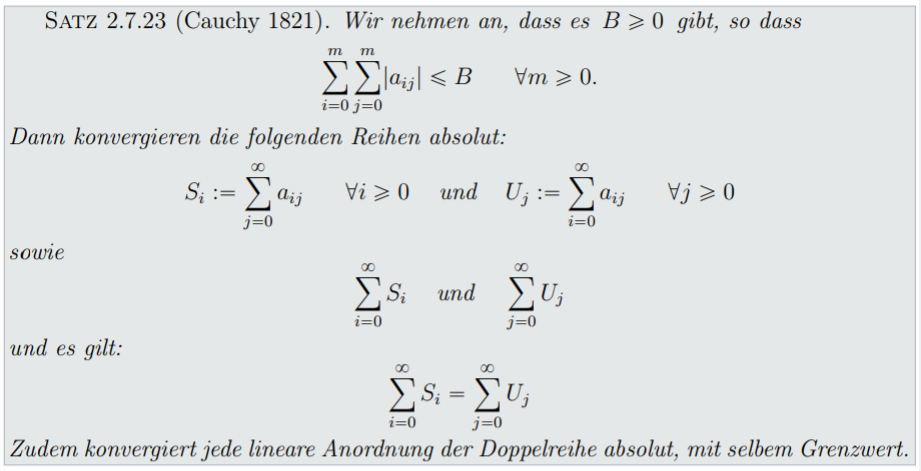
\includegraphics[width = \linewidth, scale =1]{Analysis1pic1.png}
  \caption{}
  \label{pic1}
\end{figure}
\paragraph{\underline{Potenz Reihe:}} Eine Reihe der Form:
\begin{center}
$p(x):= \displaystyle\sum_{n=0}^{\infty} a_n(x-c)^n = a_0 + a_1(x-c) + a_2(x-c)^2 + \dots$
\end{center}
wobei $a_n$ eine beliebige folge ist und $x \in \mathbb{R}$ eine parameter.
\paragraph{\underline{Konvergenz Radius:}} Der konvergenz radius einer Potenzreihe ist gegeben durch:
\begin{center}
\[
\rho := sup\{|x|: p(x) converges \}
	\begin{cases}
	\lim\limits_{n \to \infty}\big| \frac{a_n}{a_{n+1}} \big| \quad \text{ (i) Quotientenkriterium }  \\
	\frac{1}{\lim\limits_{n \to \infty} | \sqrt[n]{a_n} |} \quad \text{ (ii) Wurzelkriterium}\\
	\end{cases}
\] 

\[
|x|:=
\begin{cases}
 	< \rho \Rightarrow konvergiert \\
	> \rho \Rightarrow divergiert\\
	= \rho \Rightarrow keine \ Aussage \quad (\ast) \\
\end{cases}
\]
$(\ast):$ in diesem Fall müssen wir kontrollieren ob es konvergiert oder divergiert 
\end{center}
\paragraph{\underline{Cauchy-Produkt:}} der Reihen
\begin{center}
$\displaystyle\sum_{i = 0}^{\infty}a_i, \quad \displaystyle\sum_{j=0}^{\infty} b_j$
\end{center}
ist die Reihe
\begin{center}
$\displaystyle\sum_{n=0}^{\infty}\bigg(\displaystyle\sum_{j=0}^{n}a_{n-j}b_j \bigg) = a_0b_0 + (a_0b_1 + a_1b_0) +(a_0b_2 + a_1b_1 + a_2b_0) + \dots$
\end{center}
Falls die Reihen absolut konvergieren, so konvergiert ihr Cauchy Produkt und es gilt:
\begin{center}
$\displaystyle\sum_{n=0}^{\infty}\bigg( \displaystyle\sum_{j=0} ^{n}a_{n-j}b_j \bigg) = \bigg( \displaystyle\sum_{i=0}^{\infty}a_i \bigg) \bigg(\displaystyle\sum_{j=0}^{\infty}b_j\bigg)$
\end{center}
\paragraph{\underline{Satz 2.7.28:}} Sei $f_n : \mathbb{N} \rightarrow \mathbb{R}$ eine Folge. Wir nehmen an, dass:
\begin{enumerate}
\item f(j):= $\lim\limits_{n \to  \infty}f_n(j)$ existiert    $\forall j \in \mathbb{N}$
\item Es gibt eine Funktion $g: \mathbb{N} \rightarrow [0,\infty [$, so dass:
\begin{enumerate}
\item $ |f_n(j)| \leq g(j) \quad \forall j \geq 0 , \forall n \geq 0$
\item $\displaystyle\sum_{j=0}^{\infty}g(j)$ konvergiert
\end{enumerate}
\end{enumerate}
Dann folgt:
\begin{center}
$\displaystyle\sum_{j=0}^{\infty} f(j) = \lim\limits_{n \to \infty}\displaystyle\sum_{j=0}^{\infty} f_n(j)$
\end{center}
\chapter{Stetige Funktionen}
\section{Reelwertige Funktionen}
\paragraph{\underline{ Die Menge $\mathbb {R}^D$:}} Sei D eine beliebige Menge. Die Menge $\mathbb{R}^D$ aller Funktionen
\begin{center}
$f_ D \rightarrow \mathbb{R}$
\end{center}
bildet ein VR über $\mathbb{R}$ mit:
\begin{center}
$(f_1 + f_2)(x) = f_1(x) + f_2(x)$\\
$(\alpha \cdot f)(x) = \alpha \cdot f(x)$\\
$(f_1 \cdot f_2)(x) = f_1(x)\cdot f_2(x)$\\
$\mathit{0}(x)  = 0 \quad \forall x \in D$\\
$\mathit{1}(x) = 1 \quad \forall x \in D$\\
$ f + \mathit{0} = f, \quad g \cdot \mathit{1} = g \quad  \forall f,g \in \mathbb{R}^D$\\
Falls $|D| \geq 2$ gibt es immer ein $f \neq \mathit{0}$ das kein multiplikatives Inverses besitzt\\
$ f \leq g \text{ falls } f(x) \leq g(x) \quad \forall x \in D$\\
f ist nicht negativ falls $0\leq f$
\end{center}
\paragraph{\underline{Beschränktheit:}} Sei $f \in \mathbb{R}^D$
\begin{enumerate}
\item f ist \textbf{nach oben beschränkt}, falls $f(D) \subset \mathbb{R}$ nach oben beschränkt ist
\item f ist \textbf{nach unten beschränkt}, falls $f(D) \subset \mathbb{R}$ nach unten beschränkt ist
\item f ist \textbf{beschränkt}, falls $f(D) \subset \mathbb{R}$ beschränkt ist.
\end{enumerate}
\paragraph{\underline{Monotonie:}} $f: D \rightarrow \mathbb{R}$, wobei $D \subset \mathbb{R} falls $ $\forall x,y \in D$
\begin{enumerate}
\item \textbf{monoton wachsend} $ x\leq y \Rightarrow f(x) \leq f(y)$
\item \textbf{streng monoton wachsend} $ x<y \Rightarrow f(x) < f(y)$
\item \textbf{monoton fallend} $ x \leq y \Rightarrow f(x)  \geq f(y)$
\item \textbf{streng monoton fallend} $ x<y \Rightarrow f(x) > f(y)$
\item \textbf{monoton} falls f monoton wachsend oder monoton fallend ist
\item \textbf{steng monoton} falls f streng monoton wachsend oder streng monoton fallend ist
\end{enumerate}
\underline{Beispiel:} Sei $n \in \mathbb{N} \quad f: \mathbb{R} \rightarrow \mathbb{R} \quad x \mapsto x^n$. f ist genau dann (streng) monoton wachsend, falls n ungerade ist.
\section{Stetigkeit}
\paragraph{\underline{Stetigkeit in $x_0$:}} Sei $D \subset \mathbb{R}, x_0 \in D$. Die Funktion $f: D \rightarrow \mathbb{R}$ ist in $x_0$ stetig, falls es für jedes $\epsilon > 0$ ein $\delta > 0$ gibt so dass für alle $x \in D$ die Implikation:
\begin{center}
$|x-x_0| < \delta \Rightarrow |f(x) -f(x_0)| < \epsilon$
\end{center}
gilt.
\paragraph{\underline{Stetigkeit:}} Die Funktion $ f: D \rightarrow \mathbb{R}$ ist stetig, falls sie in jedem Punkt von D stetig ist.
\paragraph{\underline{Satz 3.2.4:}} Sei $x_0 \in D \subset \mathbb{R}$ und $ f: D \rightarrow \mathbb{R}$. Die Funktion f ist genau dann in $x_0$ stetig, falls für jede Folge ($a_n$) in D folgende Implikation gilt:
\begin{center}
$\lim\limits_{n \to \infty} a_n = x_0 \Rightarrow \lim\limits_{n \to \infty} f(a_n) = f(x_0)$
\end{center}
\paragraph{\underline{Korollar 3.2.5:}} Sei $x_0 \in D \subset \mathbb{R}, \lambda \in \mathbb{R}$ und $f:D \rightarrow \mathbb{R}, g: D \rightarrow \mathbb{R}$ beide stetig in $x_0$:
\begin{enumerate}
\item Dann sind $f + g, \lambda \cdot f, f\cdot g$ stetig in $x_0$
\item Falls $g(x_0) \neq 0$ dann ist 
\begin{center}
$\frac{f}{g} : D \cap \{x \in D : g(x) \neq 0\} \rightarrow \mathbb{R}$\\
$x \mapsto \frac{f(x)}{g(x)}$
\end{center}
stetig in $x_0$
\end{enumerate}
\paragraph{\underline{polynomiale Funktion:}} $P: \mathbb{R} \rightarrow \mathbb{R}$ ist eine Funktion der Form
\begin{center}
$P(x) = a_nx^n+ \dots + a_0$
\end{center}
wobei: $a_n, \dots, a_0 \in \mathbb{R}.$ Falls $a_n \neq 0$ ist n der \textbf{Grad} von P.\\
Polynomiale Funktionen sind auf ganz $\mathbb{R}$ stetig.\\
Seien P,Q polynomiale Funktionen auf $ \mathbb{R}$ mit Q $\neq \mathit{0}$. Seien $x_1,\dots,x_m$ die Nullstellen von Q. Dann ist:
\begin{center}
$\frac{P}{Q} : \mathbb{R} \ \{x_1,\dots x_m\} \rightarrow \mathbb{R}$\\
$ x \mapsto \frac{P(x)}{Q(x)}$

\end{center}
stetig.
\section{Der Zwischenwertsatz}
\paragraph{\underline{Satz 3.3.1 Bolzano:}} Sei $I \subset \mathbb{R}$ ein Intervall $f:I \rightarrow \mathbb{R}$ eine stetige Funktion und $a,b \in I$. Für jedes c zwischen f(a) und f(b) gibt es ein z zwischen a und b mit f(z) = c.
\paragraph{\underline{Korollar 3.3.2:}} Sei $P(x) = a_nx^n + a_{n-1}x^{n-1} + \dots + a_0$ ein Polynom mit $a_n \neq 0$ und n ungerade. Dann besitzt P mindestens eine Nullstelle in $\mathbb{R}$\\
Für c$>$ 0 besitzt $Q(x) = x^2 + c$ keine Nullstelle in $\mathbb{R}$

\paragraph{TEST:}b lbaldkajsldkfj adasdsd























\end{document}	